\documentclass[IEEEtran,letterpaper,10pt,titlepage,fleqn,draftclsnofoot,onecolumn]{article}
%notitlepage vs titlepage
%fleqn left align

%\usepackage{nopageno} %no page numbers
\usepackage{indentfirst}
\usepackage{alltt}                                           
\usepackage{float}
\usepackage{color}
\usepackage{url}

\usepackage{graphicx}                                        
\usepackage{amssymb}                                         
\usepackage{amsmath}                                         
\usepackage{amsthm}                                          

\usepackage{balance}
%\usepackage[TABBOTCAP, tight]{subfigure}
\usepackage{enumitem}
\usepackage{pstricks, pst-node}
\usepackage{geometry}
\usepackage{hyperref}
\usepackage{textcomp}
\usepackage{listings}
%allows for code snipets

\geometry{textheight=9.5in, textwidth=7in} 

\newcommand{\cred}[1]{{\color{red}#1}} %think function call, changes text to red
\newcommand{\cblue}[1]{{\color{blue}#1}} %text to blue
\definecolor{dkgreen}{rgb}{0,0.6,0}
\definecolor{gray}{rgb}{0.5,0.5,0.5}
\definecolor{mauve}{rgb}{0.58,0,0.82}
\lstset{frame=tb,
  language=c,
  aboveskip=3mm,
  belowskip=3mm,
  showstringspaces=false,
  columns=flexible,
  basicstyle={\small\ttfamily},
  numbers=none,
  numberstyle=\tiny\color{gray},
  keywordstyle=\color{blue},
  commentstyle=\color{dkgreen},
  stringstyle=\color{mauve},
  breaklines=true,
  breakatwhitespace=true,
  tabsize=3
}

\def\name{Brandon Ellis, Jiayu Han, and Jack Neff}
\def\class{CS 461 }
\def\assignment{Requirements}

%PDF Properties
\hypersetup{
  colorlinks = true,
  urlcolor = black,
  pdfauthor = {\name},
  pdfkeywords = {cs461 ``Senior Capstone' Requirements},
  pdftitle = {\class \assignment},
  pdfsubject = {\class \assignment},
  pdfpagemode = UseNone
}

\begin{document}
%TitlePage
\begin{titlepage}
	\begin{center}
		\vspace*{1cm}
		
		\huge
		\textbf{Green Smart Gardening System: Requirements}
        
        \vspace{1.5cm}
        
		\large
        \textbf{Brandon Ellis, Jiayu Han, and Jack Neff}
		
		\vspace{5cm}
    
    \normalsize
    The purpose of this document is to describe the requirements that must be fulfilled for our Green Smart Gardening System to be considered complete. It includes design requirements, such as environmental sensors; performance requirements, which dictate things like the frequency of environmental sampling; and client requirements, specifically the use of solar power.
		
		\vfill
        
		\large
        CS 461\\
        Fall Term\\
    \end{center}
\end{titlepage}

\section{Introduction}

Our Green Smart Gardening System(GSGS) will be a prototype of a green energy powered Internet-of-Thing device focusing on the environmental condition monitoring and collecting by using multiple sensors with a micro-controller. The system will transfer the collected data to a computer for analyzing and helping user to adjust the factors.

\subsection{Definitions}

\begin{itemize}
  \item GSGS - Green Smart Gardening System
  \item IOT  - Internet-of-Things
\end{itemize}

\subsection{Overview}

The rest of this document will cover a more in depth discussion of further requirements. Initially, this will be broken into two larger topics. The first topic is the Overall Description. It will touch on Product Perspective, the device need storage to store data and computer to analyze and display data; Product Functions, the device monitoring the gardening factors and help user to adjust those factors; User Characteristics, which will be from beginning level users to industries; Constraints, the device need to be waterproof and large battery capacity because of the weather in Oregon; and Assumptions \& Dependencies, what our backup plans are for analyzing and scheduling.

\vspace{5mm}

Second is the topic of Specific Requirements. It will include the Client Requirements, that it needs to be powered by solar energy; Customer User Stories, what users want from this device for both individual and industries; Technical Requirements, the ranking of importance for all sections of this project; Project Timeline, our estimated progress schedule; and Stretch Goals, some features we may want to add after the project is done. 

\section{Overall Description}
\subsection{Product Perspective}
\subsubsection{User Interface}

The user interface will provide the user with information about their garden. This will display information from all the sensors in a variety of relevant ways. Users will be able to view the current status of the garden in real time, as well as a record of periodical updates that the system will be continuously sending. In addition, algorithms we write will analyze this record and try to find correlations between data sets that can be displayed to the user in graphical form.   

\subsubsection{Hardware Devices}

The hardware devices required are a microcontroller with internet capability, and an array of sensors that can connect to the microcontroller. A solar power source is required, as well as a battery capable of lasting through the typical overcast season in the Willamette Valley. Access to a computer will be necessary for analysis and viewing of the data, as to not require the user to physically check the device.

\subsubsection{Memory Operations}

We will need a database to store packets of environmental information in, and for ease of access when analyzing it. The sensors themselves do not need memory, but the microcontroller should probably have a limited amount of memory, in case the internet connection goes bad. If it can store several packets in memory, it can stockpile those packets and transmit them when the connection is restored.  

\subsubsection{Site Adaptation Requirements}

We will need to construct a garden and seed some plants, recording environmental data and plant growth data over a period of time. We will need a bed of soil with adequate drainage and sunlight, and places to install all the environmental sensors we want to use. The location must also have an internet connection, so the data can be relayed to the database from the microcontroller. 

\subsection{Product Functions}

The Green Smart Gardening System (Working Title) is a data collection and analysis system for vineyards. It uses sensors of a variety of environmental conditions connected to a centralized microcontroller to analyze patterns of plant growth. We will use proprietary algorithms to analyze and display this data to users. Hopefully, when the gardening system has collected enough information, it will be able to suggest increases or decreases of water application based on current conditions. On a large scale, this system will monitor berry farms or vineyards, help their owner manage them, and possibly connect to other similar systems in the area in order to gather more data and get more accurate readings. 

\subsection{User Characteristics}

The original use case for this device was framed around the Southern Oregon Wine Industry. We intend for it to stay true to that in making our device accessible to a more amatuer user, while broadening the use to recreational as well as industrial gardening. Users will be assumed to be beginner level skill in both gardening and computer usage. Accordingly, the interface must be simple and intuitive, and as helpful as possible with tips to increase plant growth and maintain optimal conditions.   

\subsection{Constraints}
\subsubsection{Safety}

Due to the fact that we plan on having a device that can perform in the elements, there needs to be some care given to ensuring it can do this safely. We can addresses this in two separate ways. First, we can protect connections between the device and sensors. This will prevent potentially hazardous shorts and improve the longevity of our device. Second, components that do not require interaction with the elements can be put in a housing device. This will make sure that at least the microcontroller and battery are not unnecessarily exposed to wear. 

\subsubsection{Hardware}

Our chief software constraints are in the vein of power supply. We have decided to implement a solar component into the system, so when possible, the system will run on solar power and use any excess energy collected to charge its battery. Oregon’s Willamette Valley, where we envision this product, sees significantly reduced sunlight during the Winter. This affects the battery sizes we will use, which must be made large enough to support their components through these months. In addition to larger batteries, sensors and the microcontroller will need to be as efficient as possible, transmitting information at relatively long intervals. The other main constraint besides power for the microcontroller is the memory. The more storage, the more power use, but also the better backed-up information is if there is something wrong with the connection.   

\subsection{Assumptions}

We assume that the sensors we select will be able to interact with our microcontroller. If not, we will need to replace the sensors or microcontroller. We assume we will be able to collect data in a synchronous way with multiple sensors. If not, we will need to design more complex analysis algorithms, which will take more time. We will, based on calculations, assume our battery setup will last from installation well into the Spring of 2018. If not we need to recalculate and either increase battery life or decrease power usage. We assume we will be able to algorithmically analyze the best way to treat a plant based on data.If not, we may need to do some research on plants and develop a more educated approach.  

\clearpage

\section{Specific Requirements}
\subsection{Client Requirements}

A key requirement that our clients are asking for is that our device is powered through green method. The specific method requested is solar. To this end our device will have a solar panel that will feed into a rechargeable battery, fulfilling our client’s requirement and ensuring that our device is sustainable and does not require constant battery changes.

\subsection{Customer User Stories}

\begin{itemize}
  \item As the owner of a garden, I can check the environmental data of my garden so that I can make informed decisions about my plants’ health.
  \item As the user of a smart gardening device, I can access my device in such a way that it is intuitive to use.
  \item As the owner of a smart gardening device, I can trust that my device will have a sustainable power system such that I do not have to switch batteries frequently.
  \item As the owner of an industrial farm, I know my device can weather the elements such that I don’t have to perform maintenance and replace parts.
  \item As a smart gardening device user, I can view the data of my garden in such a way that it is easily accessible and readable without having to physically check the device.
\end{itemize}

\subsection{Technical Requirements}

The following is a list of hierarchical requirements to create the base version of our device. The element of hierarchy dictates which requirements are dependent on their predecessors. This information is also shown in the form of a Gantt chart below. 

\begin{itemize}
  \item Assemble board, sensors, wireless output method, and provide solar power to the device.
  \item Create software interfaces between sensors and board.
  \item Ensure collected data from sensors can be saved to an SD card.
  \item Establish connection between wireless device and external storage system.
  \item Validate that retrieved data matches confirmed environmental conditions.
  \item Create a user interface that outputted data can be viewed through.
\end{itemize}

\subsection{Project Timeline}

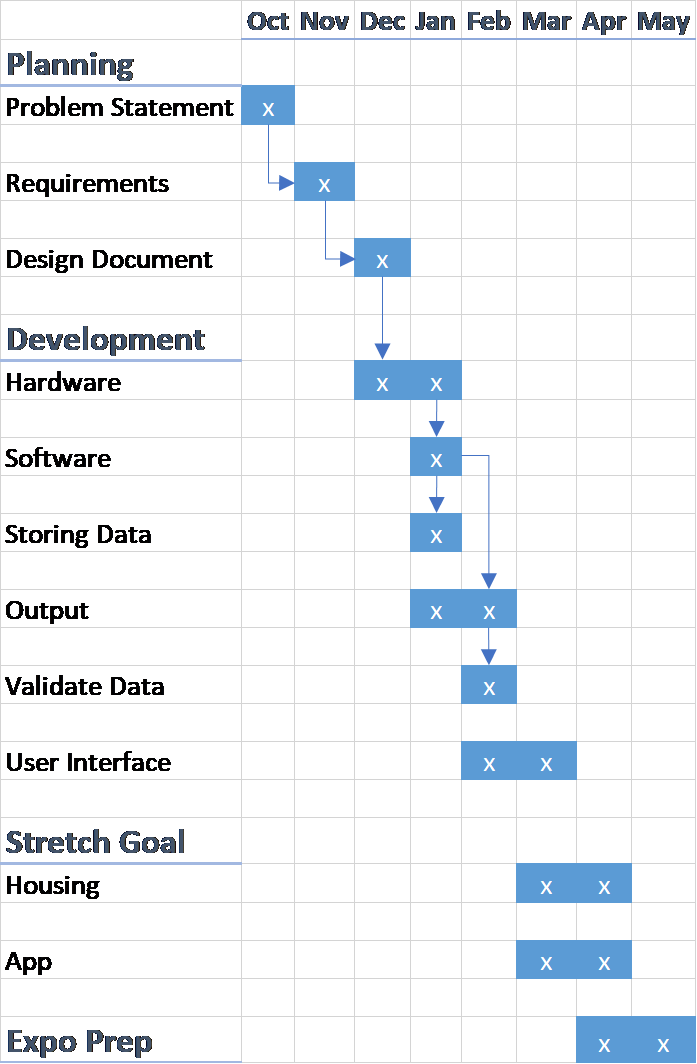
\includegraphics{Gantt_Chart}

\subsection{Stretch Goals}

When all of the base requirements have been established, there are a couple stretch goals that can be attained. The first is a housing for the created device. This would protect it from the elements, with the exception of sensors that would require being external. Additionally, it would be a finalizing touch to have the sensitive internal device contained within one protective unit. The second goal is the creation of an app. This app would enable the user to view their data in a much more mobile manner. The app would connect to whatever database is utilized to house what the device has outputted.

\end{document}